\begin{abcliste}
\abc Die mittlere Geschwindigkeit ist die Ortsänderung geteilt durch die Zeit. Die Ortsänderung ist die Fläche unter dem $v(t)$-Graphen, ein Dreieck und ein Rechteck:
\begin{align}
 \Delta s &= \dsF = \frac{1}{2}\cdot\vMax\cdot\tOne+\vMax\cdot\left(\tE-\tOne\right) = \ds \\
 \bar v &= \vMeanF = \frac{\ds}{\tE} = \vMean \approx \result{\vMeanP{0}{1}}
\end{align}
Im Diagramm ist $\bar v$ die Höhe des Rechtecks, das über derselben Zeit dieselbe Fläche hat wie die Fläche unter dem Graphen (rot gestrichelt):
\begin{center}
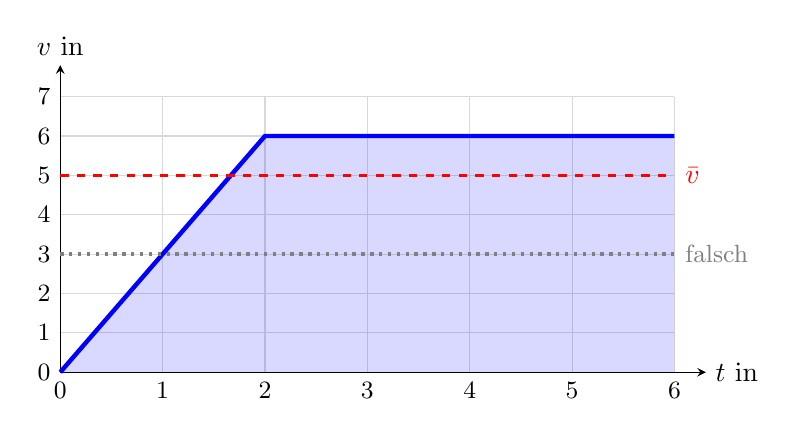
\begin{tikzpicture}[>=stealth, x=1.3cm, y=0.5cm]
 \draw[gray!30] (0,0) grid[xstep=1, ystep=1] (6,7);
 \draw[->] (0,0) -- (6.308,0) node[right] {$t$ in \si{\second}};
 \draw[->] (0,0) -- (0,7.8) node[above] {$v$ in \si{\meter\per\second}};
 \foreach \tk in {0,1,2,3,4,5,6} \node[below] at (\tk,0) {\small $\tk$};
 \foreach \yk in {0,1,2,3,4,5,6,7} \node[left] at (0,\yk) {\small $\yk$};

 \fill[blue, opacity=0.15] (0,0) -- (2,6) -- (6,6) -- (6,0) -- cycle;
 \draw[ultra thick, blue] (0,0) -- (2,6) -- (6,6);
 \draw[very thick, red, dashed] (0,5) -- (6,5) node[right] {$\bar v$};
 \draw[very thick, gray, dotted] (0,3) -- (6,3) node[right] {\small falsch};
\end{tikzpicture}
\end{center}
\abc Sara mittelt nur die Anfangs- und die Endgeschwindigkeit: $\vWrongP{0}{1}$. Das ist $\result{\text{nur richtig, wenn } v(t) \text{ eine einzige Gerade ist}}$ (gleichmässige Beschleunigung während der ganzen Zeit). Hier fährt das Auto nur \tOneO\ lang langsamer als \SI{6}{\meter\per\second}, die übrigen \SI{4}{\second} aber mit \SI{6}{\meter\per\second}. Die mittlere Geschwindigkeit liegt deshalb näher bei \SI{6}{\meter\per\second}. Mit \vWrongP{0}{1} wäre das Auto in \tEO\ nur \SI{18}{\meter} weit gekommen statt \dsP{0}{2}.
\end{abcliste}
